\section{Tecniche utilizzate}

Vengono ora presentate le tecniche utilizzate all'interno del programma: l'estrazione di \emph{features} dall'immagine mediante l'utilizzo dei \emph{filtri di Gabor} e il Descrittore di Covarianza (\emph{Covariance Descriptor}).

\subsection{Il filtro di Gabor}

I filtri di Gabor\footnote{Gabor, D.: \emph{Theory of communication.} In J. IEE, vol. 93, pp. 429-457, Londra, 1946.} sono filtri passa-banda usati nell'analisi di immagini principalmente per l'estrazione di \emph{features} e l'analisi basata sulla tessitura.

La risposta finita all'impulso di questi filtri è calcolata come prodotto di uno sviluppo Gaussiano con oscillazione complessa. Estendendo queste funzioni a due dimensioni è possibile creare filtri sensibili all'orientazione\footnote{Daugman, J. G.: \emph{Uncertainty relation for resolution in space, spatial frequency, and orientation optimized by two-dimensional visual cortical filters} J. Optical Society of America A, vol. 2, no. 7, pp. 1160-1169, July 1985.} e sotto certe condizioni è possibile approssimare linearmente la fase.

Sia $(x, y)$ un punto dell'immagine. L'equazione per il filtro di Gabor 2D è la seguente:

$$G(x, y) = e^{(- \frac{(x')^2 + \gamma^2 (y')^2}{2 \sigma^2})} \cos (2 \pi \frac{x'}{\lambda})  $$ 

con 

$$x' = x \cos \theta + y \sin \theta$$
$$y' = - x \cos \theta + y \sin \theta$$

I parametri del filtro sono:
\begin{itemize}
\item $\theta$: orientazione del filtro, espressa in gradi.
\item $\lambda$: lunghezza d'onda del fattore coseno, espressa in pixels.
\item $\gamma$: specifica l'ellitticità del supporto della funzione di Gabor.
\item $\sigma$: è il parametro che regola l'inviluppo Gaussiano.
\end{itemize}

\begin{figure}[H] 
  \centering
    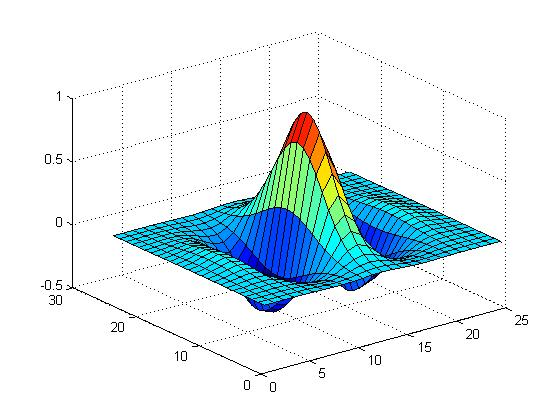
\includegraphics[width=0.5\textwidth]{images/gaborfilter.jpg}
    \vspace{-0.5cm}
    \caption{{\small \textit{Esempio di filtro di Gabor 2D}}}
\end{figure}

Al fine di estrarre utili \emph{features} da un'immagine è utile utilizzare un set di filtri di Gabor con parametri diversi, ad esempio la scala e l'orientazione.

Nel programma viene utilizzato un set di filtri di Gabor con 4 diverse angolazioni e 3 diverse scale per un totale di 12 filtri:

\begin{figure}[H] 
  \centering
    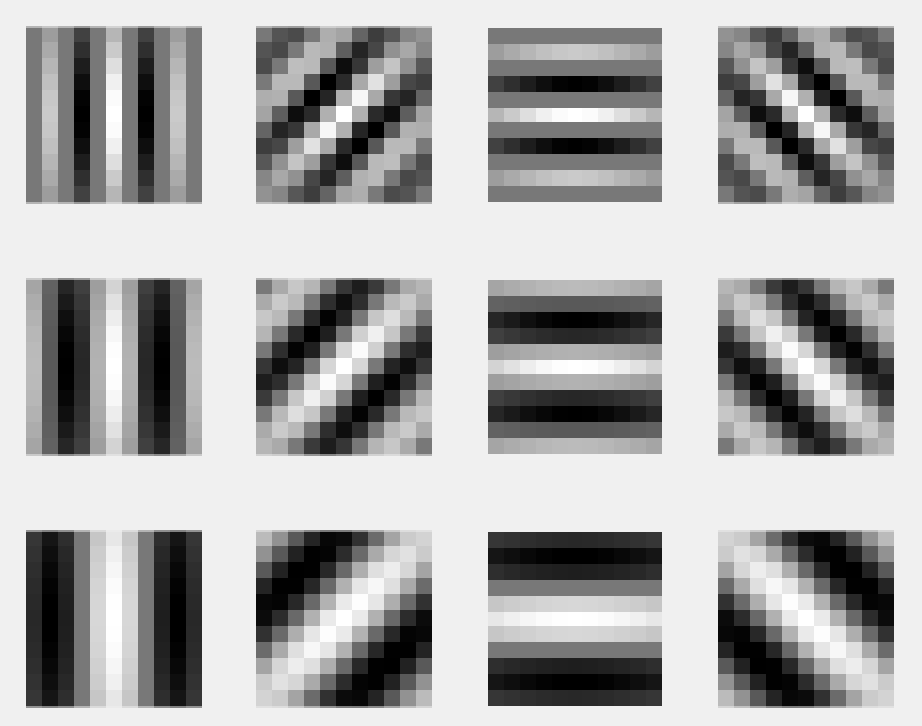
\includegraphics[width=0.5\textwidth]{images/filterbank.png}
    \caption{{\small \textit{Set di filtri di Gabor con 4 angolazioni e 3 scale}}}
\end{figure}

Per ciascun pixel dell'immagine viene dunque calcolato il vettore delle \emph{features} ottenute mediante la convoluzione dell'immagine con i filtri di Gabor (dividendo la parte reale dalla parte immaginaria).

\subsection{Descrittore di Covarianza}

Il Descrittore di Covarianza (Covariance Descriptor\footnote{Oncel Tuzel, Fatih Porikli, Peter Meer, \emph{Region Covariance: A Fast Descriptor for
Detection and Classification} Mitsubishi Electric Research Laboratories, Inc., 2006.}, CovD) viene utilizzato in letteratura per descrivere e caratterizzare regioni di immagini. 

Data un'immagine con associato, a ciascun pixel, un vettore di \emph{features}, il Descrittore di Covarianza codifica informazioni che riguardano le \emph{varianze} di queste ultime all'interno di una regione, la loro correlazione e la loro distribuzione nello spazio. Questo metodo è molto utilizzato in particolare modo quando si ha bisogno di rimanere invarianti rispetto all'illuminazione o alla rotazione.

Data un'immagine $I$ con associato, per ciascun pixel $(x, y)$, il vettore di features di dimensione $d$, si considera $F$ come l'immagine di features a $d$ livelli. Viene dunque considerata una regione di F tale che $R \subset F$ e consideriamo $\{f_i\}_{i = 1,\ldots, n} \in R$ la $i$-esima features, con $n$ numero di pixels della regione.

A questo punto la regione $R$ viene rappresentata da una matrice di covarianza di dimensione $d X d$ dei \emph{features points}:

$$C = \frac{1}{n -1} \sum_{k = 1}^{n} (f_k - \mu)(f_k - \mu)^T$$

con $\mu$ la media dei \emph{features points}.

Poichè la matrice $C$ è definita positiva e simmetrica può essere considerata un \emph{tensore}. Il problema principale è che lo spazio del tensore così definito non è uno spazio Euclideo. Per questo la varietà della covarianza viene spesso definita Riemanniana per determinare un insieme di strumenti efficaci della geometria differenziale.

\subsection{Tensori di Fisher}

I \emph{tensori di Fisher} rappresentano la controparte definita su varietà Riemanniana dei \emph{vettori di Fisher}.

Il vettore di Fisher (\emph{FV}) è una rappresentazione di una immagine ottenuta raccogliendo osservazioni locali dall'immagine stessa. E' usato comunemente come un descrittore globale di immagini nella classificazione.

Sia $I = (x_1, \ldots, x_N)$ un insieme composto da $N$ vettori di $D$ osservazioni (\emph{features vectors}) estratte dall'immagine. Siano poi $G = (\mu_k, \Sigma_k, \pi_k; k = 1, \ldots, K)$ i parametri di un Modello a Mistura di Gaussiane (\emph{GMM}) opportuno per la distribuzione dei descrittori.

Il GMM associa ciascun vettore $x_i$ a uno stato $k$:

$$ q_{ik} = \frac{e^{-\frac{1}{2} (x_i - \mu_k)^T \Sigma_{k}^{-1}(x_i - \mu_k)}}{\sum_{t = 1}^{K} e^{-\frac{1}{2} (x_i - \mu_t)^T \Sigma_{k}^{-1}(x_i - \mu_t)}}$$

Per ciascuna moda $k$ consideriamo il vettore media ed il vettore di covarianza della deviazione:

$$u_{ik} = \frac{1}{N\sqrt{\pi_k}} \sum_{i = 1}^{N} q_{ik} \frac{x_{ji} - \mu_{jk}}{\sigma_{jk}}$$
$$v_{jk} = \frac{1}{N\sqrt{2 \pi_k}} \sum_{i = 1}^{N} q_{ik} [\frac{x_{ji} - \mu_{jk}}{\sigma_{jk}}^2 - 1]$$

con $j = 1, \ldots, D$.

Il FV di un immagine I è la concatenazione dei vettori $u_k$ e $v_k$ per ciascuno dei $K$ stati del GMM

$$FV(I) = \left[
     \begin{array}{c}
     u_1 \\ \vdots \\ u_K \\ v_1 \\ \vdots \\ v_K 
     \end{array}
     \right]$$
